\documentclass[10pt,a4paper]{article}
\usepackage[utf8]{inputenc}
\usepackage[T1]{fontenc}
\usepackage[romanian]{babel}
\usepackage[margin=1.7cm]{geometry}
\usepackage{amsmath,amssymb,mathtools}
\usepackage{enumitem}
\usepackage{titlesec}
\usepackage{parskip}
\usepackage{tikz}
\usetikzlibrary{calc,arrows.meta,positioning}
\usepackage{pgfplots}
\pgfplotsset{compat=1.18}
\usepackage[most]{tcolorbox}
\usepackage{xcolor}

\newtcolorbox{res}{colback=red!6,colframe=red!65!black,boxrule=0.6pt,arc=1.5pt,
  left=4pt,right=4pt,top=2pt,bottom=2pt,breakable}

\setlist{nosep, topsep=2pt, itemsep=2pt, leftmargin=1.3em}
\titlespacing*{\section}{0pt}{6pt}{2pt}
\titlespacing*{\subsection}{0pt}{4pt}{1pt}
\renewcommand{\baselinestretch}{0.96}
\setlength{\parindent}{0pt}
\pagestyle{empty}

\begin{document}
\begin{center}
{\large\bfseries Rezolvare --- Model de antrenament SAE}
\end{center}
\vspace{-0.2cm}

\section*{1. $G(s)=\dfrac1{s(s+5)}$, $T_e=0.1$s}

\subsection*{a) Funcția de transfer în circuit închis (metoda trapezului)}
$$\color{blue}s=\frac{2}{T_e}\cdot\frac{z-1}{z+1}=20\,\frac{z-1}{z+1}$$
$$s+5=\frac{20(z-1)+5(z+1)}{z+1}=\frac{25z-15}{z+1}=\frac{5(5z-3)}{z+1}$$
$$G(z)=\frac1{s(s+5)}=\frac{(z+1)^2}{20(z-1)\cdot5(5z-3)}=\frac{(z+1)^2}{100(z-1)(5z-3)}=\frac{z^2+2z+1}{500z^2-800z+300}$$
$$H(z)=\frac{G(z)}{1+G(z)}=\frac{z^2+2z+1}{(500z^2-800z+300)+(z^2+2z+1)}$$
\begin{res}
$$H(z)=\frac{(z+1)^2}{501z^2-798z+301}$$
\end{res}

\subsection*{b) Eroare staționară}
$$K_p=\lim_{z\to1}G(z)=\infty\qquad
K_v=\frac1{T_e}\lim_{z\to1}(z-1)G(z)=\frac1{T_e}\cdot\frac{(z+1)^2}{100(5z-3)}\bigg|_{z=1}=\frac1{0.1}\cdot\frac4{200}=0.2$$
$$K_a=\frac1{T_e^2}\lim_{z\to1}(z-1)^2G(z)=0$$
\begin{res}
$$e_{ss}(\text{treaptă})=\frac1{1+K_p}=0\qquad
e_{ss}(\text{rampă})=\frac1{K_v}=\frac1{0.2}=5\qquad
e_{ss}(\text{parabolă})=\frac1{K_a}=\infty$$
\end{res}

\subsection*{c) Răspunsul la impuls unitar Dirac}
$$R(z)=1\ \Rightarrow\ Y(z)=H(z)$$
$$z_{1,2}=\dfrac{798\pm\sqrt{798^2-4\cdot501\cdot301}}{1002}=\dfrac{798\pm40\sqrt{21}}{1002}$$
$$z_1\approx0.9793\qquad z_2\approx0.6135\quad(\text{sistem stabil})$$
$$\frac{Y(z)}{z}=\frac{z^2+2z+1}{z(501z^2-798z+301)}=\frac{A}{z}+\frac{B}{z-z_1}+\frac{C}{z-z_2}$$
$$A=\frac{N(0)}{D(0)}=\frac1{301}\approx0.0033,\qquad
B=\frac{N(z_1)}{z_1\cdot501(z_1-z_2)}\approx0.0218,\qquad
C=\frac{N(z_2)}{z_2\cdot501(z_2-z_1)}\approx-0.0232$$
$$N(z)=(z+1)^2,\quad D(z)=501z^2-798z+301$$
$$Y(z)=A+\frac{Bz}{z-z_1}+\frac{Cz}{z-z_2}$$
\begin{res}
$$Y(z)=0.0033+\frac{0.0218\,z}{z-0.9793}-\frac{0.0232\,z}{z-0.6135}$$
\end{res}
$$\textcolor{blue}{\mathcal Z^{-1}\{1\}=\delta(k),\qquad \mathcal Z^{-1}\{z/(z-a)\}=a^k u(k)}$$
\begin{res}
$$y(k)=0.0033\,\delta(k)+0.0218\,(0.9793)^k-0.0232\,(0.6135)^k,\quad k\ge0$$
\end{res}
Verificare: $\sum_k y(k)=H(1)=\dfrac{4}{501-798+301}=\dfrac44=1$, câștig static unitar — consistent cu $e_{ss}(\text{treaptă})=0$.

\begin{center}
\begin{tabular}{@{}rrrrrrrrr@{}}
$k$ & 0&1&2&3&4&5&6&7\\
$y(k)$ & 0.0020&0.0072&0.0122&0.0152&0.0168&0.0177&0.0180&0.0181\\[2pt]
$k$ & 8&9&10&11&12&13&14&15\\
$y(k)$ & 0.0180&0.0178&0.0175&0.0172&0.0169&0.0166&0.0163&0.0159\\
\end{tabular}
\end{center}

\begin{center}
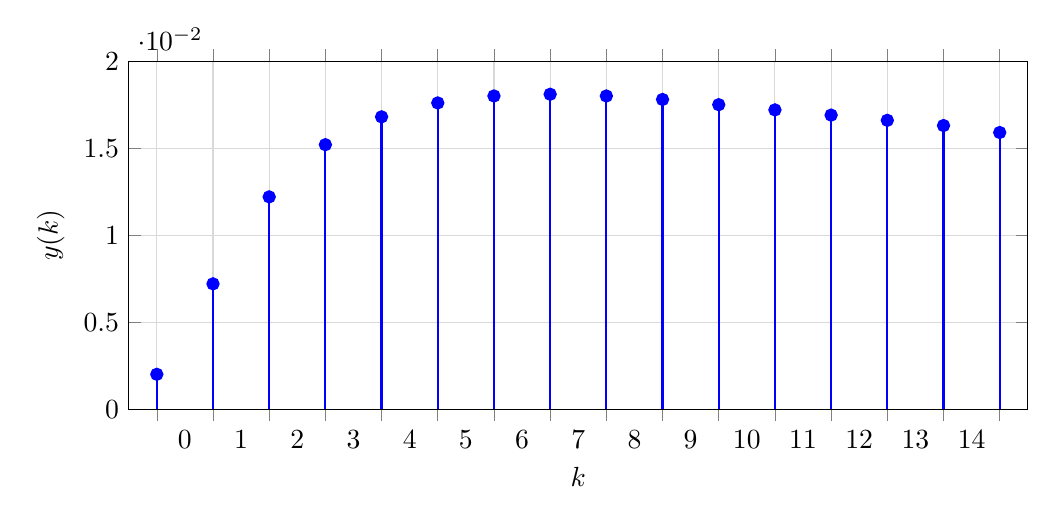
\begin{tikzpicture}
\begin{axis}[
  width=13cm,height=6cm,
  xlabel={$k$}, ylabel={$y(k)$},
  xmin=-0.5,xmax=15.5, ymin=0, ymax=0.0200,
  grid=both, minor grid style={gray!15}, major grid style={gray!30},
  ybar interval, bar width=6pt,
]
\addplot[ycomb,thick,blue,mark=*,mark options={fill=blue}] coordinates {
(0,0.0020)(1,0.0072)(2,0.0122)(3,0.0152)(4,0.0168)(5,0.0176)
(6,0.0180)(7,0.0181)(8,0.0180)(9,0.0178)(10,0.0175)(11,0.0172)
(12,0.0169)(13,0.0166)(14,0.0163)(15,0.0159)
};
\end{axis}
\end{tikzpicture}
\end{center}

\section*{2. $G_d(z)=\dfrac{0.2z+0.07}{z^2-0.5z+0.05}$, $T_e=1$s (circuit deschis, reacție unitară)}
$$\color{blue}z=\frac{1+\frac{T_e}2w}{1-\frac{T_e}2w}\overset{T_e=1}{=}\frac{1+0.5w}{1-0.5w}=\frac ND,\ N=1{+}0.5w,\ D=1{-}0.5w$$
$$0.2z+0.07=\frac{0.2N+0.07D}D=\frac{0.27+0.07w}D$$
$$z^2-0.5z+0.05=\frac{N^2-0.5ND+0.05D^2}{D^2}=\frac{0.39w^2+0.95w+0.55}{D^2}$$
\begin{res}
$$G_d(w)=\frac{(0.27+0.07w)\,D}{0.39w^2+0.95w+0.55}=\frac{-0.03w^2-0.07w+0.27}{0.39w^2+0.95w+0.55}$$
\end{res}
$$N(w)=0\Rightarrow w_{z1}=2,\quad w_{z2}=-4.15\qquad D(w)=0\Rightarrow w_{p1}=-0.94,\quad w_{p2}=-1.51$$
\begin{res}
$$G_d(w)=\underbrace{\frac{0.27}{0.55}}_{K_B=0.49}\cdot\frac{\left(1-\dfrac w2\right)\left(1+\dfrac w{4.15}\right)}{\left(1+\dfrac w{0.94}\right)\left(1+\dfrac w{1.51}\right)}$$
\end{res}
$w_{z1}=2>0\Rightarrow$ zerou neminim-fazic.
Frecvențe de frângere (rad/s): $\omega_{p1}=0.94,\ \omega_{p2}=1.51,\ \omega_{z1}=2,\ \omega_{z2}=4.15$.
\begin{res}
Panta asimptotică a modulului (nivel de start $20\lg K_B=-6.18$dB):
$$\underbrace{0}_{\omega<0.94}\to\underbrace{-20}_{0.94<\omega<1.51}\to\underbrace{-40}_{1.51<\omega<2}\to\underbrace{-20}_{2<\omega<4.15}\to\underbrace{0}_{\omega>4.15}\ \text{dB/dec}$$
Nivel final ($\omega\to\infty$): $20\lg\left|\dfrac{-0.03}{0.39}\right|=-21.53$dB (raport coeficienți dominanți).
Fază asimptotică ($\omega\to\infty$): $2\text{ poli}(-90^\circ)+1\text{ zerou m.f.}(+90^\circ)+1\text{ zerou n.m.f.}(-90^\circ)=-180^\circ$.
\end{res}
\begin{res}
\begin{center}
\begin{tabular}{@{}rrrrrrrrrr@{}}
$\omega$&0.01&0.1&0.5&1&2&5&10&50&100\\
$|G_d|_{dB}$&$-6.18$&$-6.24$&$-7.39$&$-9.84$&$-14.09$&$-19.14$&$-20.80$&$-21.50$&$-21.52$\\
$\varphi\,[^\circ]$&$-1.1$&$-11.4$&$-53.5$&$-93.3$&$-137.0$&$-170.5$&$-177.3$&$-179.7$&$-179.8$\\
\end{tabular}
\end{center}
\end{res}

\begin{center}
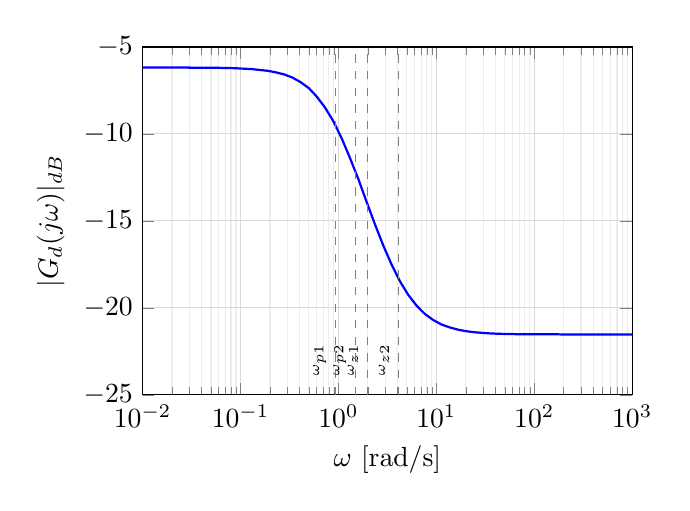
\begin{tikzpicture}
\begin{semilogxaxis}[
  width=7.8cm,height=6cm,
  xlabel={$\omega$ [rad/s]}, ylabel={$|G_d(j\omega)|_{dB}$},
  xmin=0.01,xmax=1000, ymin=-25,ymax=-5,
  grid=both, minor grid style={gray!15}, major grid style={gray!30},
]
\addplot[blue,thick] coordinates {
(0.01,-6.18) (0.01,-6.18) (0.01,-6.18) (0.02,-6.18) (0.02,-6.18) (0.03,-6.18) (0.03,-6.19) (0.04,-6.19) (0.05,-6.19) (0.06,-6.20) (0.07,-6.21) (0.09,-6.22) (0.10,-6.24) (0.13,-6.27) (0.15,-6.31) (0.19,-6.37) (0.23,-6.46) (0.28,-6.58) (0.34,-6.76) (0.41,-7.02) (0.50,-7.37) (0.60,-7.85) (0.73,-8.48) (0.89,-9.28) (1.08,-10.25) (1.31,-11.37) (1.60,-12.60) (1.94,-13.90) (2.36,-15.19) (2.87,-16.41) (3.49,-17.51) (4.24,-18.46) (5.15,-19.24) (6.26,-19.86) (7.61,-20.34) (9.25,-20.69) (11.24,-20.95) (13.66,-21.12) (16.61,-21.25) (20.19,-21.34) (24.54,-21.40) (29.82,-21.44) (36.25,-21.47) (44.06,-21.49) (53.56,-21.50) (65.10,-21.51) (79.12,-21.52) (96.17,-21.52) (116.9,-21.52) (142.08,-21.52) (172.7,-21.52) (209.91,-21.53) (255.14,-21.53) (310.12,-21.53) (376.94,-21.53) (458.16,-21.53) (556.88,-21.53) (676.88,-21.53) (822.72,-21.53) (1000,-21.53)
};
\addplot[gray,dashed] coordinates {(0.94,-25)(0.94,-5)};
\addplot[gray,dashed] coordinates {(1.51,-25)(1.51,-5)};
\addplot[gray,dashed] coordinates {(2,-25)(2,-5)};
\addplot[gray,dashed] coordinates {(4.15,-25)(4.15,-5)};
\node[above,rotate=90,font=\tiny] at (axis cs:0.94,-23) {$\omega_{p1}$};
\node[above,rotate=90,font=\tiny] at (axis cs:1.51,-23) {$\omega_{p2}$};
\node[above,rotate=90,font=\tiny] at (axis cs:2,-23) {$\omega_{z1}$};
\node[above,rotate=90,font=\tiny] at (axis cs:4.15,-23) {$\omega_{z2}$};
\end{semilogxaxis}
\end{tikzpicture}
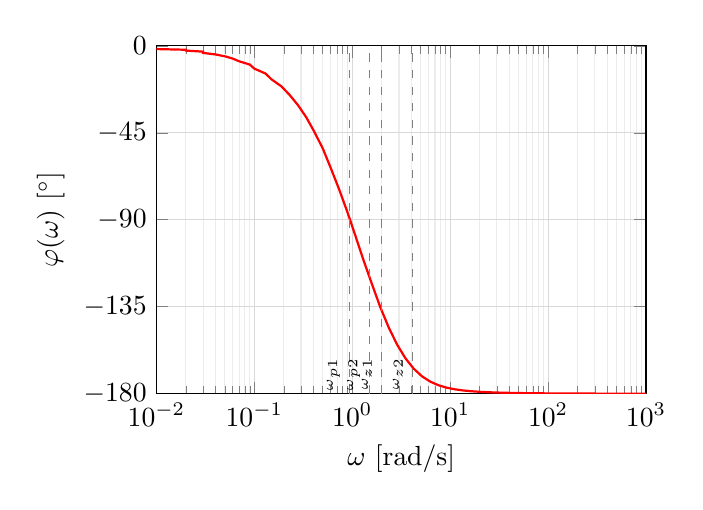
\begin{tikzpicture}
\begin{semilogxaxis}[
  width=7.8cm,height=6cm,
  xlabel={$\omega$ [rad/s]}, ylabel={$\varphi(\omega)$ [$^\circ$]},
  xmin=0.01,xmax=1000, ymin=-180,ymax=0,
  ytick={-180,-135,-90,-45,0},
  grid=both, minor grid style={gray!15}, major grid style={gray!30},
]
\addplot[red,thick] coordinates {
(0.01,-1.14) (0.01,-1.38) (0.01,-1.68) (0.02,-2.04) (0.02,-2.48) (0.03,-3.02) (0.03,-3.67) (0.04,-4.46) (0.05,-5.42) (0.06,-6.58) (0.07,-8.00) (0.09,-9.72) (0.10,-11.80) (0.13,-14.32) (0.15,-17.37) (0.19,-21.06) (0.23,-25.48) (0.28,-30.78) (0.34,-37.07) (0.41,-44.48) (0.50,-53.08) (0.60,-62.91) (0.73,-73.88) (0.89,-85.82) (1.08,-98.41) (1.31,-111.21) (1.60,-123.70) (1.94,-135.38) (2.36,-145.77) (2.87,-154.56) (3.49,-161.63) (4.24,-167.03) (5.15,-170.97) (6.26,-173.74) (7.61,-175.63) (9.25,-176.90) (11.24,-177.75) (13.66,-178.33) (16.61,-178.74) (20.19,-179.02) (24.54,-179.23) (29.82,-179.39) (36.25,-179.51) (44.06,-179.60) (53.56,-179.67) (65.10,-179.73) (79.12,-179.78) (96.17,-179.82) (116.9,-179.85) (142.08,-179.88) (172.7,-179.90) (209.91,-179.92) (255.14,-179.93) (310.12,-179.94) (376.94,-179.96) (458.16,-179.96) (556.88,-179.97) (676.88,-179.97) (822.72,-179.98) (1000,-179.98)
};
\addplot[gray,dashed] coordinates {(0.94,-180)(0.94,0)};
\addplot[gray,dashed] coordinates {(1.51,-180)(1.51,0)};
\addplot[gray,dashed] coordinates {(2,-180)(2,0)};
\addplot[gray,dashed] coordinates {(4.15,-180)(4.15,0)};
\node[above,rotate=90,font=\tiny] at (axis cs:0.94,-170) {$\omega_{p1}$};
\node[above,rotate=90,font=\tiny] at (axis cs:1.51,-170) {$\omega_{p2}$};
\node[above,rotate=90,font=\tiny] at (axis cs:2,-170) {$\omega_{z1}$};
\node[above,rotate=90,font=\tiny] at (axis cs:4.15,-170) {$\omega_{z2}$};
\end{semilogxaxis}
\end{tikzpicture}
\end{center}

\section*{3. $G_d(z)=\dfrac{k(0.13z+0.02)}{z^2-0.39z+0.007}$, $T_e=1$s}
Poli: $z^2-0.39z+0.007=0\Rightarrow p_{1,2}=\dfrac{0.39\pm\sqrt{0.39^2-4\cdot0.007}}{2}$
\begin{res}
$$p_1=0.37\qquad p_2=0.02\qquad z_0=-\frac{0.02}{0.13}=-0.15\ (\text{zero})$$
\end{res}

\subsection*{a) Numărul de ramuri}
$n=2$, $m=1\Rightarrow$ nr. ramuri $=\max(n,m)=2$.
\begin{res}
Ramuri din $p_1=0.37$, $p_2=0.02$; se termină în $z_0=-0.15$ și în $z\to\infty$.
\end{res}

\subsection*{b) Porțiunea de pe axa reală}
\begin{res}
$$(p_2,\,p_1)=(0.02,\,0.37)\qquad\text{și}\qquad(-\infty,\,z_0)=(-\infty,\,-0.15)$$
\end{res}

\subsection*{c) Asimptote}
$$n-m=1,\qquad \textcolor{blue}{\theta=\frac{180^\circ(2k+1)}{n-m}}=180^\circ$$
$$\textcolor{blue}{\sigma_a=\frac{\sum p_i-\sum z_i}{n-m}}=\frac{(0.37+0.02)-(-0.15)}{1}=0.54$$
\begin{res}
1 asimptotă, $180^\circ$, $\sigma_a=0.54$.
\end{res}

\subsection*{d) Punctele de ramificație}
$$\color{blue}k(z)=-\frac{N(z)}{D(z)},\qquad \frac{dk}{dz}=0$$
$$N(z)=z^2-0.39z+0.007,\quad D(z)=0.13z+0.02$$
$$0.13z^2+0.04z-0.01=0$$
\begin{res}
$$z_{b1}=0.15\ (k\approx0.73)\qquad
z_{b2}=-0.45\ (k\approx10.0)$$
\end{res}

\subsection*{e) Verificare cerc \& trasare}
$$\color{blue}z=z_0+w:\quad w^2+w\big[2z_0-p_1-p_2+k\big]+(z_0-p_1)(z_0-p_2)=0$$
$$\color{blue}|w|^2=w\bar w=(z_0-p_1)(z_0-p_2)\quad(\text{independent de }k)$$
$$r=\sqrt{(z_0-p_1)(z_0-p_2)}=\sqrt{(-0.15-0.37)(-0.15-0.02)}$$
\begin{res}
$$r=\sqrt{0.52\cdot0.17}=0.30$$
Verificare: $|z_{b1}-z_0|=0.30$ și $|z_{b2}-z_0|=0.30$ — exact raza.
\end{res}

\begin{center}
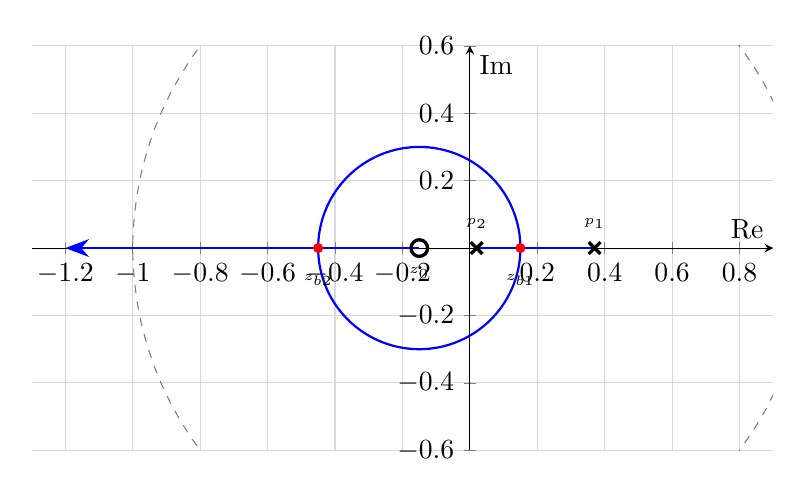
\begin{tikzpicture}
\begin{axis}[
  width=11cm,height=9cm,
  xlabel={$\mathrm{Re}$}, ylabel={$\mathrm{Im}$},
  xmin=-1.3,xmax=0.9,ymin=-0.6,ymax=0.6,
  axis equal image,
  axis lines=middle,
  grid=both, minor grid style={gray!15}, major grid style={gray!30},
]
\addplot[gray,dashed,domain=0:360,samples=100] ({cos(x)},{sin(x)});
\addplot[blue,thick,domain=0:360,samples=200] ({-0.15+0.30*cos(x)},{0.30*sin(x)});
\addplot[blue,thick] coordinates {(0.02,0)(0.15,0)};
\addplot[blue,thick] coordinates {(0.15,0)(0.37,0)};
\addplot[blue,thick] coordinates {(-0.45,0)(-0.15,0)};
\addplot[blue,thick,-{Stealth[length=3mm]}] coordinates {(-0.45,0)(-1.2,0)};
\addplot[only marks,mark=x,black,mark size=3pt,line width=1.2pt] coordinates {(0.37,0)(0.02,0)};
\addplot[only marks,mark=o,black,mark size=3pt,line width=1.2pt] coordinates {(-0.15,0)};
\addplot[only marks,mark=*,red,mark size=1.6pt] coordinates {(0.15,0)(-0.45,0)};
\node[above] at (axis cs:0.37,0.03) {\tiny $p_1$};
\node[above] at (axis cs:0.02,0.03) {\tiny $p_2$};
\node[below] at (axis cs:-0.15,-0.03) {\tiny $z_0$};
\node[below] at (axis cs:0.15,-0.05) {\tiny $z_{b1}$};
\node[below] at (axis cs:-0.45,-0.05) {\tiny $z_{b2}$};
\end{axis}
\end{tikzpicture}
\end{center}
(cerc punctat = cerc unitate.)

\section*{4. $G_0(z)=\dfrac{0.02z+0.02}{z^2-1.49z+0.54}$}

\subsection*{a) Model la stare, forma complet controlabilă}
$$\textcolor{blue}{G_0(z)=\frac{Y(z)}{U(z)}=\frac{b_1z+b_0}{z^2+a_1z+a_0}},\qquad a_1=-1.49,\ a_0=0.54,\ b_1=0.02,\ b_0=0.02$$
$$\color{blue}w(k+2)-a_1\,w(k+1)+a_0\,w(k)=u(k),\qquad y(k)=b_1\,w(k+1)+b_0\,w(k)$$
$$w(k+2)=1.49\,w(k+1)-0.54\,w(k)+u(k)$$
$$\color{blue}x_1(k)=w(k),\quad x_2(k)=w(k+1)$$
$$x_1(k+1)=x_2(k)\qquad x_2(k+1)=-0.54\,x_1(k)+1.49\,x_2(k)+u(k)\qquad y(k)=0.02\,x_1(k)+0.02\,x_2(k)$$
\begin{res}
$$A=\begin{pmatrix}0&1\\-0.54&1.49\end{pmatrix},\quad B=\begin{pmatrix}0\\1\end{pmatrix},\quad C=\begin{pmatrix}0.02&0.02\end{pmatrix},\quad D=0$$
\end{res}
$$AB=\begin{pmatrix}1\\1.49\end{pmatrix},\quad \textcolor{blue}{Q_c=\begin{pmatrix}B & AB\end{pmatrix}}=\begin{pmatrix}0&1\\1&1.49\end{pmatrix},\quad \det Q_c=-1\ne0\ \Rightarrow\ \text{complet controlabil}$$

\subsection*{b) Observabilitate}
$$CA=\begin{pmatrix}0.02&0.02\end{pmatrix}\begin{pmatrix}0&1\\-0.54&1.49\end{pmatrix}=\begin{pmatrix}-0.0108&0.0498\end{pmatrix}$$
\begin{res}
$$Q_o=\begin{pmatrix}C\\CA\end{pmatrix}=\begin{pmatrix}0.02&0.02\\-0.0108&0.0498\end{pmatrix},\qquad \det Q_o=0.02\cdot0.0498-0.02\cdot(-0.0108)=0.0012\ne0$$
Sistemul este \textbf{complet observabil}.
\end{res}

\section*{5. $G(z)=\dfrac{z^2-1.39z+0.52}{z^2-1.43z+0.49}$}

\subsection*{a) Model la stare, forma complet observabilă}
$$\textcolor{blue}{G(z)=\frac{Y(z)}{U(z)}=\frac{b_2z^2+b_1z+b_0}{z^2+a_1z+a_0}},\qquad a_1=-1.43,\ a_0=0.49,\ b_2=1,\ b_1=-1.39,\ b_0=0.52$$
$$B(z)-b_nA(z)=(z^2-1.39z+0.52)-(z^2-1.43z+0.49)=0.04z+0.03=B'(z)$$
$$D=b_n=1,\qquad b_1'=b_1-b_na_1=-1.39-(-1.43)=0.04,\qquad b_0'=b_0-b_na_0=0.52-0.49=0.03$$
$$\textcolor{blue}{G(z)=D+\frac{B'(z)}{A(z)}}=1+\frac{0.04z+0.03}{z^2-1.43z+0.49}$$
$$\color{blue}x_1(k+1)=-a_0x_2(k)+b_0'u(k)\qquad x_2(k+1)=x_1(k)-a_1x_2(k)+b_1'u(k)\qquad y_{sp}(k)=x_2(k)$$
$$y(k)=x_2(k)+Du(k)$$
\begin{res}
$$A_o=\begin{pmatrix}0&-a_0\\1&-a_1\end{pmatrix}=\begin{pmatrix}0&-0.49\\1&1.43\end{pmatrix},\quad
B_o=\begin{pmatrix}b_0'\\b_1'\end{pmatrix}=\begin{pmatrix}0.03\\0.04\end{pmatrix},\quad
C_o=\begin{pmatrix}0&1\end{pmatrix},\quad D=1$$
\end{res}
Verificare: $(zI-A_o)=\begin{pmatrix}z&0.49\\-1&z-1.43\end{pmatrix}$, $\det=z^2-1.43z+0.49=A(z)$ $\checkmark$.
$$C_o(zI-A_o)^{-1}B_o=\frac{[0\ \ 1]\begin{pmatrix}z-1.43&-0.49\\1&z\end{pmatrix}\begin{pmatrix}0.03\\0.04\end{pmatrix}}{z^2-1.43z+0.49}=\frac{0.03+0.04z}{z^2-1.43z+0.49}$$
$$G(z)=C_o(zI-A_o)^{-1}B_o+D=1+\frac{0.04z+0.03}{z^2-1.43z+0.49}=\frac{z^2-1.39z+0.52}{z^2-1.43z+0.49}\quad\checkmark$$
$$C_oA_o=\begin{pmatrix}0&1\end{pmatrix}\begin{pmatrix}0&-0.49\\1&1.43\end{pmatrix}=\begin{pmatrix}1&1.43\end{pmatrix}$$
\begin{res}
$$Q_o=\begin{pmatrix}C_o\\C_oA_o\end{pmatrix}=\begin{pmatrix}0&1\\1&1.43\end{pmatrix},\quad\det Q_o=0\cdot1.43-1\cdot1=-1\ne0\ \Rightarrow\ \text{complet observabil}$$
\end{res}

\subsection*{b) Schema bloc}
$$x_1(k+1)=-0.49\,x_2(k)+0.03\,u(k)\qquad x_2(k+1)=x_1(k)+1.43\,x_2(k)+0.04\,u(k)\qquad y(k)=x_2(k)+u(k)$$

\begin{center}
\begin{tikzpicture}[>=Stealth, font=\small]
\node[draw,circle,minimum size=6mm] (SA) at (3,0) {};
\draw (SA.north west) -- (SA.south east) (SA.north east) -- (SA.south west);
\node[draw,minimum width=12mm,minimum height=8mm] (Z1) at (5,0) {$z^{-1}$};
\node[draw,circle,minimum size=6mm] (SB) at (7.2,0) {};
\draw (SB.north west) -- (SB.south east) (SB.north east) -- (SB.south west);
\node[draw,minimum width=12mm,minimum height=8mm] (Z2) at (9.4,0) {$z^{-1}$};
\node[draw,circle,minimum size=6mm] (SY) at (11.6,0) {};
\draw (SY.north west) -- (SY.south east) (SY.north east) -- (SY.south west);

\node (uin) at (-1.3,0) {$u(k)$};
\node (yout) at (13.2,0) {$y(k)$};

\coordinate (ubranch) at (-0.3,0);
\draw[->] (uin) -- (ubranch);
\fill (ubranch) circle (1.3pt);
\draw[->] (ubranch) -- (SA);
\draw[->] (SA) -- (Z1);
\draw[->] (Z1) -- (SB) node[midway,above]{\tiny$x_1(k)$};
\draw[->] (SB) -- (Z2);
\coordinate (xtap) at (10.9,0);
\draw[->] (Z2) -- (SY) node[midway,above]{\tiny$x_2(k)$};
\fill (xtap) circle (1.3pt);
\draw[->] (SY) -- (yout);

\draw (ubranch) -- (-0.3,2.2) -- (11.6,2.2);
\draw[->] (3,2.2) -- (SA) node[midway,right]{\tiny$b_0'=0.03$};
\draw[->] (7.2,2.2) -- (SB) node[midway,right]{\tiny$b_1'=0.04$};
\draw[->] (11.6,2.2) -- (SY) node[midway,right]{\tiny$D=1$};

\draw (xtap) -- (10.9,-2.2) -- (3,-2.2);
\draw[->] (3,-2.2) -- (SA) node[midway,left]{\tiny$-a_0=-0.49$};
\draw[->] (7.2,-2.2) -- (SB) node[midway,left]{\tiny$-a_1=1.43$};
\end{tikzpicture}
\end{center}
(formă canonică observabilă — Direct Form II transpusă.)

\section*{Teorie (pe scurt)}

\subsection*{1. Transformarea planului $s$ în planul $z$}
$$\color{blue}x^*(t)=\sum_k x(kT_e)\delta(t-kT_e),\qquad X^*(s)=\sum_k x(kT_e)e^{-skT_e}\quad(\text{periodică, }j\omega_e=j2\pi/T_e)$$
$$\color{blue}z=e^{sT_e}:\quad \mathrm{Re}(s)=0\to|z|=1,\qquad \mathrm{Re}(s)<0\to|z|<1$$

\subsection*{2. Schema bloc a unui sistem de reglare numeric}
$$\color{blue}R(z)\to\text{Sumator}(\pm)\to H_R(z)\to\text{N/A+ZOH}\to G(s)\to y(t)\to\text{A/N}\to(\text{reacție})$$

\subsection*{3. Etapele conversiei analog-numerice}
$$\color{blue}\text{Eșantionare}\to\text{Reținere (S\&H)}\to\text{Cuantizare}\to\text{Codificare}$$

\subsection*{4. Elementele specifice unui sistem numeric}
A/N (ADC), regulator numeric, N/A (DAC) + ERO/ZOH, eșantionator (perioadă $T_e$).

\subsection*{5. Eșantionorul ideal în schemă bloc}
$$\color{blue}x^*(t)=x(t)\sum_k\delta(t-kT_e)$$

\end{document}
